\documentclass[conference]{IEEEtran}
\IEEEoverridecommandlockouts
% The preceding line is only needed to identify funding in the first footnote. If that is unneeded, please comment it out.
\usepackage{cite}
\usepackage{amsmath,amssymb,amsfonts}
\usepackage{algorithmic}
\usepackage{graphicx}
\usepackage{textcomp}
\usepackage{xcolor}
\usepackage{gensymb}
\usepackage{listings}
\usepackage[framed,numbered,autolinebreaks,useliterate]{mcode}
\def\BibTeX{{\rm B\kern-.05em{\sc i\kern-.025em b}\kern-.08em
    T\kern-.1667em\lower.7ex\hbox{E}\kern-.125emX}}
\begin{document}

\title{RBE 501 Week 6: Physics by EL Assignment}

\author{\IEEEauthorblockN{Arjan Gupta}
\IEEEauthorblockA{\textit{Robotics Engineering} \\
\textit{Worcester Polytechnic Institute}\\
Worcester, MA, USA \\
agupta11@wpi.edu}
}

\maketitle

\begin{abstract}
This document provides an in-depth solution for the Week 6 Physics by Euler-Lagrange problems in RBE 501.\\
\end{abstract}

\begin{IEEEkeywords}
physics, euler-lagrange equations
\end{IEEEkeywords}

\section{Introduction}
For Week 6, we are given two problems. The first problem shows us a mass $m$ that is free to
move on the surface of a frictionless table. Mass $m$ is attached to another mass $M$ via a
string that goes through a hole in the table. We can assume the string has no spring-like
properties, and is therefore always taut. The representation of this system is shown in 
Figure~\ref{problem-1-given-fig}. Our first objective in this problem is to solve for the Euler-Lagrange
equations of this system with respect to $r$ and $\theta$. Our second and third objectives here
are to discuss the behaviors of $r$ and $\theta$ in the EL equations. The fourth objective of the
first problem is to give the conditions under which $\dot{r}$ and $\ddot{r}$ cause a circular motion
for mass $m$.\\

\begin{figure}[h!]
    \centering
    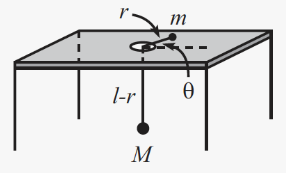
\includegraphics[scale=0.35]{problem-1-given-fig.png}
    \caption{Given figure for Problem 1}
    \label{problem-1-given-fig}
\end{figure}

The second problem shows a mass $m$ that is held at rest on ramp of mass $M$. The ramp has inclination
$\theta$, as shown in Figure \ref{problem-2-given-fig}. The surface of the ramp is frictionless, and the
surface upon which the ramp rests is also frictionless. Our objective is to find the acceleration of
the ramp caused by the release of mass $m$, and we must use Euler-Lagrange approach for this.

\begin{figure}
    \centering
    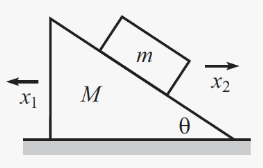
\includegraphics[scale=0.35]{problem-2-given-fig.png}
    \caption{Given figure for Problem 2}
    \label{problem-2-given-fig}
\end{figure}

\section{Materials and Methods}

\subsection{Approach for Problem I}

Our first step toward solving Problem I is to find the overall kinetic energy ($T$) and
overall potential energy ($U$) of the system. We then find the Lagrangian of the system
as $L = T - U$. We can then use the Euler-Lagrangian equation,

\begin{equation} \label{prob1_eq_motion_r}
    \frac{d}{dt} \left(\frac{\partial L}{\partial \dot{r}}\right) = \frac{\partial L}{ \partial r}
\end{equation}
and
\begin{equation} \label{prob1_eq_motion_theta}
    \frac{d}{dt} \left(\frac{\partial L}{\partial \dot{\theta}}\right) = \frac{\partial L}{ \partial \theta}
\end{equation}

to discuss the behaviors of $r$ and $\theta$.\\

\subsubsection{Find overall kinetic energy of the system ($T$)}
In Fig. 1, we consider vector $\textbf{r}$. Say the \textit{x-y} plane is the surface
of the table. Since we consider an angle $\theta$ as shown, we can say,

\[
    \textbf{r} =
    \begin{pmatrix}
        r \cos \theta\\
        r \sin \theta
    \end{pmatrix}
\]

Where the magnitude of $r$ is dependent on theta. Differentiating
with respect to $\theta$ to get velocity,

\[
    \dot{\textbf{r}} =
    \begin{pmatrix}
        \dot{r} \cos \theta - r \dot{\theta} \sin \theta\\
        \dot{r} \sin \theta + r \dot{\theta} \cos \theta
    \end{pmatrix}
\]

To find the kinetic energy, we need the square of this velocity,
which is simply the dot product of the vector with itself.

\begin{align*}
    \dot{\textbf{r}}^2 = \dot{\textbf{r}} \cdot \dot{\textbf{r}}
    &= (\dot{r} \cos \theta - r \dot{\theta} \sin \theta)^2 +
    (\dot{r} \sin \theta + r \dot{\theta} \cos \theta)^2\\
    &= \dot{r}^2 \cos^2 \theta + r^2 \dot{\theta}^2 \sin^2 \theta 
    + 2 r \dot{r} \dot{\theta} \cos\theta \sin\theta\\
    + \dot{r}^2 \sin^2 \theta + r^2 \dot{\theta}^2 \cos \theta
    - 2 r \dot{r} \dot{\theta} \cos\theta \sin\theta\\
    &= \dot{r}^2 (\cos^2\theta + \sin^2\theta) 
    + r^2\dot{\theta}^2 (\cos^2\theta + \sin^2\theta)\\
\end{align*}
Hence,
\[
    \dot{\textbf{r}}^2 = \dot{r}^2 + r^2\dot{\theta}^2
\]

Therefore the kinetic energy of the mass $m$ moving on the table is given as,

\begin{equation} \label{prob1_ke_mass_small_m}
    T_m = \frac{1}{2}~m~(\dot{r}^2 + r^2\dot{\theta}^2)
\end{equation}
Also, the length of the string that suspends 
mass $M$ is $l-r$, where
total length of the string is $l$. The suspended part
of the string is also along the axes perpendicular to the table,
which is the \textit{z} axis. Therefore, the kinetic energy of the
mass $M$ moving perpendicular to the table is given as

\begin{equation} \label{prob1_ke_mass_big_m}    
    T_M = \frac{1}{2}~M~\left(\frac{d}{dt}(l-r)\hat{\textbf{z}}\right)^2 = \frac{1}{2}~M~\dot{r}^2
\end{equation}

So, using Equations~\ref{prob1_ke_mass_small_m} and~\ref{prob1_ke_mass_big_m},
the total kinetic energy of the system ($T$) is,

\begin{align*}
    T &= T_m + T_M\\
      &=\frac{1}{2}~m~(\dot{r}^2 + r^2\dot{\theta}^2) + \frac{1}{2}~M~\dot{r}^2
\end{align*}
Rearranging,
\begin{equation} \label{prob1_overall_ke}
    T = \frac{1}{2} \dot{r}^2 (m + M) + \frac{1}{2} m r^2 \dot{\theta}^2
\end{equation}

\subsubsection{Find overall potential energy of system}
The potential energy is also a sum of the potential energies of the masses
$m$ and $M$ in the system. The only source of potential energy in
this system is gravity caused by the earth. Since we are free to define
the reference point from where we can count the height from earth, let us
define the table-top in Figure~\ref{problem-1-given-fig} as height $h = 0$.
Also, $g$ is the constant acceleration due to gravity.

This means,

\[
    U_m = mgh = mg~(0) = 0
\]

and,

\[
    U_M = Mg(-(l-r)) = -Mg(r-l)
\]

So, the overall potential energy of the system is simply,
\begin{equation} \label{prob1_overall_pe}
    U = U_M + U_m = -Mg(r-l)
\end{equation}

\subsubsection{Find Lagrangian of the system}
The Lagrangian of the system is given as $L = T - U$. Using Equations 
\ref{prob1_overall_ke} and \ref{prob1_overall_pe}, we get

\begin{align*}
    L &= \left(\frac{1}{2} \dot{r}^2 (m + M) + 
        \frac{1}{2} m r^2 \dot{\theta}^2\right) -
        (-Mg(r-l))\\
    L &= \frac{1}{2} \dot{r}^2 (m + M) + 
    \frac{1}{2} m r^2 \dot{\theta}^2 + Mg(r-L)
\end{align*}

\subsubsection{Find equations of motion for the system}
Using Equations \ref{prob1_eq_motion_r} and \ref{prob1_eq_motion_theta}
to find the equations of motion.

\subsection{Approach for Problem 3--5}

\subsubsection{Restate objective in technical terms}
In technical terms, we must first assign frames 0 through 3 for
each link of the manipulator. We will then form a table of DH
parameters. Using the table, and the general form of the DH matrix,
we will find the $A$ matrices for the manipulator i.e.\ we need to find
$A_1$, $A_2$, and $A_3$. Using these, we need to find $T^0_3$
to give us our final answer. From our textbook~\cite{Spong2006}, the 
DH Coordinate Frame Assumptions are,
\begin{itemize}
    \item \textbf{(DH1)} The axis $x_i$ is perpendicular to the axis $z_{i-1}$.
    \item \textbf{(DH2)} The axis $x_i$ intersects the axis $z_{i-1}$.
\end{itemize}
\vspace{0.1in}
\vspace{0.1in}
\subsubsection{Assign frames}
The first step toward solving our problem is to redraw the robot
manipulator in symbolic
form, and assign frames for links 0 through 3. Since we are following the DH assumptions,
we must follow the frame assignment style shown in Figure 4, which
is from our textbook~\cite{Spong2006}. Our redrawn figure is shown in Figure 5.\\

As shown, frame 0 ($x_0 y_0 z_0$) is assigned at the first joint (revolute). Frame 1
($x_1 y_1 z_1$) is also assigned at the
first joint in order to have DH assumptions satisfied. Frame 2 ($x_2 y_2 z_2$)
 is assigned at third joint (revolute). Frame 3 ($x_3 y_3 z_3$) is assigned at
the end of link 3, in a way that also satisfies DH assumptions.\\

\subsubsection{Create DH table and set variables/constants}
Now that we have assigned the frames, we can use Figure 4 to write
the $\alpha_i$, $a_i$, $\theta_i$, $d_i$ quantities for each link.

\begin{table}[h!]
    \begin{center}
        \resizebox{0.8\columnwidth}{!}{%
        \begin{tabular}{||c|c|c|c|c||}
        \hline
        Link & $\alpha_i$ & $a_i$ & $\theta_i$ & $d_i$ \\
        \hline\hline
        1 & $-90\degree$ & 0 & $\theta_1$ & 0 \\
        2 & $90\degree$ & 0 & 0 & $L_1 + q_2$ \\
        3 & 0 & $L_3$ & $90\degree + \theta_3$ & 0\\
        \hline
        \end{tabular}
        }
    \end{center}
    \caption{Denavit-Hartenberg table for Problem 3--5}
\end{table}

As seen in Table 1, we have chosen $L_1$ and $L_3$ to describe the constant link
lengths of links 1 and 3, respectively. Additionally, $q_2$ describes the variable
link length of link 2 (because of joint 2 being a prismatic joint).
Furthermore, $\theta_1$ and $\theta_3$ describe the
variable angles of revolute joints 1 and 3, respectively.

\subsubsection{Find $A$ matrices}

As given in our textbook~\cite{Spong2006}, the general form of an
$A_i$ matrix is,

\[
    A_i =
    \begin{bmatrix}
        c_{\theta_i} & -s_{\theta_i}c_{\alpha_i} & s_{\theta_i}s_{\alpha_i} & a_i c_{\theta_i}\\
        s_{\theta_i} & c_{\theta_i}c_{\alpha_i} & -c_{\theta_i}s_{\alpha_i} & a_i s_{\theta_i}\\
        0 & s_{\alpha_i} & c_{\alpha_i} & d_i\\
        0 & 0 & 0 & 1
    \end{bmatrix}
\]

Where $c_{\theta_i}$ is $\cos{\theta_i}$, $s_{\theta_i}$ is $\sin{\theta_i}$,
$c_{\alpha_i}$ is $\cos{\alpha_i}$, and $s_{\alpha_i}$ is $\sin{\alpha_i}$.
We can write a MATLAB function for this $A_i$ matrix, as follows.


Using this function in our MATLAB Live Script, we produce the following A matrices.

\[
    A_1 =
    \begin{bmatrix}
        \cos \theta_1 & 0 & -\sin \theta_1 & 0\\
        \sin \theta_1 & 0 & \cos  \theta_1 & 0\\
        0 & -1 & 0 & 0\\
        0 & 0 & 0 & 1
        \end{bmatrix}
\]

\[
    A_2 = 
    \begin{bmatrix}
        1 & 0 & 0 & 0\\
        0 & 0 & -1 & 0\\
        0 & 1 & 0 & L_1 + q_2 \\
        0 & 0 & 0 & 1
        \end{bmatrix}
\]

\[
    A_3 =
    \begin{bmatrix}
        \cos \left(\theta_3 +\frac{\pi }{2}\right) & -\sin \left(\theta_3 +\frac{\pi }{2}\right) & 0 & L_3 \,\cos \left(\theta_3 +\frac{\pi }{2}\right)\\
        \sin \left(\theta_3 +\frac{\pi }{2}\right) & \cos \left(\theta_3 +\frac{\pi }{2}\right) & 0 & L_3 \,\sin \left(\theta_3 +\frac{\pi }{2}\right)\\
        0 & 0 & 1 & 0\\
        0 & 0 & 0 & 1
        \end{bmatrix}
\]

Now we are ready to multiply these matrices to obtain the final result
of our objective.

\section{Results}

\subsection{Result for Problem 3--2}

For Problem 3--2, we obtained our final result by multiplying all three $H$ matrices
that we obtained in the Materials and Methods section. Hence, we obtained the following
matrix,
\[
    H^0_3 =
    \begin{bmatrix}
        \sigma_1  & 0 & \sigma_5  & \lambda_1\\
        0 & 1 & 0 & 0\\
        \sigma_4  & 0 & \sigma_1  & \lambda_2\\
        0 & 0 & 0 & 1
    \end{bmatrix}
\]

where,
\begin{multline*}
    \lambda_1 = L_1 \,\cos \left(\theta_1 \right)+L_3 \,\cos \left(\theta_3 \right)\,\sigma_2 \\-L_3 \,\sin \left(\theta_3 \right)\,\sigma_3 +L_2 \,\cos \left(\theta_1 \right)\,\cos \left(\theta_2 \right)\\-L_2 \,\sin \left(\theta_1 \right)\,\sin \left(\theta_2 \right)
\end{multline*}
\begin{multline*}
    \lambda_2 = -L_1 \,\sin \left(\theta_1 \right)-L_3 \,\cos \left(\theta_3 \right)\,\sigma_3 -L_3 \,\sin \left(\theta_3 \right)\,\sigma_2\\ -L_2 \,\cos \left(\theta_1 \right)\,\sin \left(\theta_2 \right)-L_2 \,\cos \left(\theta_2 \right)\,\sin \left(\theta_1 \right)
\end{multline*}
and,
\begin{align*}
    \sigma_1 &=\cos \left(\theta_3 \right)\,\sigma_2 -\sin \left(\theta_3 \right)\,\sigma_3 \\
    \sigma_2 &=\cos \left(\theta_1 \right)\,\cos \left(\theta_2 \right)-\sin \left(\theta_1 \right)\,\sin \left(\theta_2 \right)\\
    \sigma_3 &=\cos \left(\theta_1 \right)\,\sin \left(\theta_2 \right)+\cos \left(\theta_2 \right)\,\sin \left(\theta_1 \right)\\
    \sigma_4 &= -\cos \left(\theta_3 \right)\,\sigma_3 -\sin \left(\theta_3 \right)\,\sigma_2\\
    \sigma_5 &= \cos \left(\theta_3 \right)\,\sigma_3 +\sin \left(\theta_3 \right)\,\sigma_2
\end{align*}

The significance of this $H^0_3$ matrix is that is provides
a direct transformation matrix between the base frame (frame 0) and end-effector frame,
which is a solution for forward kinematics.

\subsection{Result for Problem 3--5}

For Problem 3--5, we obtained our final result by multiplying all three $A_i$ matrices
that we obtained in the Materials and Methods section. Hence, we obtained the following
matrix,

\[
    T^0_3 =
    \begin{bmatrix}
        \sigma_1  & \sigma_4 & 0 & \lambda_1\\
        \sigma_5 & \sigma_1  & 0 & \lambda_2\\
        0 & 0 & 1 & 0\\
        0 & 0 & 0 & 1
    \end{bmatrix}\\
\]
where,
\begin{align*}
    \lambda_1 &= L_3 \,\cos \left(\theta_1 \right)\,\sigma_3 -\sin \left(\theta_1 \right)\,{\left(L_1 +q_2 \right)}-L_3 \,\sin \left(\theta_1 \right)\,\sigma_2\\
    \lambda_2 &= \cos \left(\theta_1 \right)\,{\left(L_1 +q_2 \right)}+L_3 \,\cos \left(\theta_1 \right)\,\sigma_2 +L_3 \,\sigma_3 \,\sin \left(\theta_1 \right)
\end{align*}
and,
\begin{align*}
    \sigma_1 &=\cos \left(\theta_1 \right)\,\sigma_3 -\sin \left(\theta_1 \right)\,\sigma_2 \\
    \sigma_2 &=\sin \left(\theta_3 +\frac{\pi }{2}\right)\\
    \sigma_3 &=\cos \left(\theta_3 +\frac{\pi }{2}\right)\\
    \sigma_4 &= -\cos \left(\theta_1 \right)\,\sigma_2 -\sigma_3 \,\sin \left(\theta_1 \right)\\
    \sigma_5 &= \cos \left(\theta_1 \right)\,\sigma_2 +\sigma_3 \,\sin \left(\theta_1 \right)
\end{align*}

The significance of this $T^0_3$ matrix is that is provides
a direct transformation matrix between the base frame (frame 0) and end-effector frame, 
which is a solution for forward kinematics.

\section{Discussion}
In the opinion of the author, this homework problem set was insightful. The
first problem proved that we do not need to always use the DH convention
when solving for forward kinematics in robotic manipulators. In fact, when
using tools like MATLAB, manually executing a non-DH method of
computing the forward kinematics is no more complex than using the DH method
itself.\\
The second problem reinforced our learnings from RBE 500. We used the DH
convention heavily in that class, so it was great to revisit that foundation
as we move forward in this class.\\
A topic for further consideration could be, when would one prefer to use
a non-DH method over the DH method? The DH convention can provide a minimal
and efficient way to represent and compute the relationship between the base
frame and the end effector in many cases, because it reduces the number of
variables involved from 6 to 4. However, suppose we want to model the
differential kinematics of a manipulator. The screw-based theory~\cite{Rocha2011}
can provide advantages in such a case. In the referenced paper for screw-based
theory, it was found that, when
various kinematic modelings for common manipulator configurations where
compared, the screw-based theory did not provide any disadvantages in any
case. The one noticeable difference was that it provided superior flexibility
when differential kinematics was compared.
The parameter identification is also a bit simpler in the screw-based theory, as
compared to the DH-convention.\\
It was a great exercise the solve this week's problem set, and the author thanks
the Professor for this.
\bibliography{refs.bib}
\bibliographystyle{IEEEtran}

\end{document}